\section{Image Quality Assessment}
To evaluate the amount of distortions in the dataset a method for \gls{iqa} is needed. A recent state of the art method is that of Deep IQA \cite{deepiqa}. Deep IQA is a \gls{cnn}-based \gls{nr} \gls{iqa} method that can be trained to measure the visual quality of an image. It is deeper than previous deep-based \gls{iqa} methods with the architecture being inspired by VGG nets \cite{vgg}. Deep IQA consists of 14 convolutional layers, 5 max-pooling layers and 2 fully-connected layers. The architecture is shown in \figref{deepiqa_arch}. The convolutional layers are all 3 $\times$ 3 convolution kernels and activated using \gls{relu}. Inputs to each convolutional layer are zero-padded to ensure output size is equal to the input. Max-pooling layers consist of 2 $\times$ 2 sized kernels. The network is trained on mini-batches of 32 $\times$ 32 patches. During inference non-overlapping patches are sampled from the image and image quality scores are predicted for each instance. The patch scores are averaged for the final score for the entire image. 

\begin{figure}[H]
  \centering
    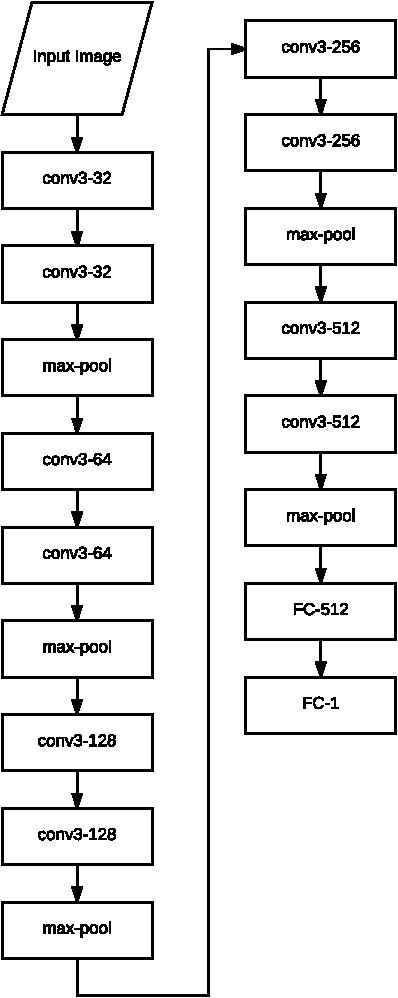
\includegraphics[width=0.3\textwidth]{Figs/Implementation/deepiqa_arch.pdf}
      \caption{Architecture of the Deep IQA network. Notation for convolutional layers are conv(receptive field size)-(number of channels) and fully-connected layers are FC(number of channels).}
    \label{fig:deepiqa_arch}
\end{figure}

Training Deep IQA requires a database of annotated images with both reference images and distorted counterparts. The following section will outline the database used in this project for \gls{iqa} training.

\subsection{LIVE Image Quality Database}
Deep IQA assesses three different datasets for this purpose. These are \gls{live} which consists of 5 different distortions \cite{livepaper}, TID2013 \cite{tid2013} with 24 different distortions and CSIQ \cite{cisq} with 5 types. For simplicity purposes the only \gls{live} dataset is chosen for this project. The dataset was made for the purposes of evaluating the subjective visual quality of images in regards to the five distortion types. The distortions are generated from 29 colour reference images that are of both high-resolution and high quality. An example of images from the dataset can be seen in \figref{live_ex}. The references image were collected to have a wide variety in different content, this includes faces, people, animals, nature and man-made objects.

\begin{figure}[H]
    \centering
    \begin{subfigure}[b]{0.4\textwidth}
        \center
        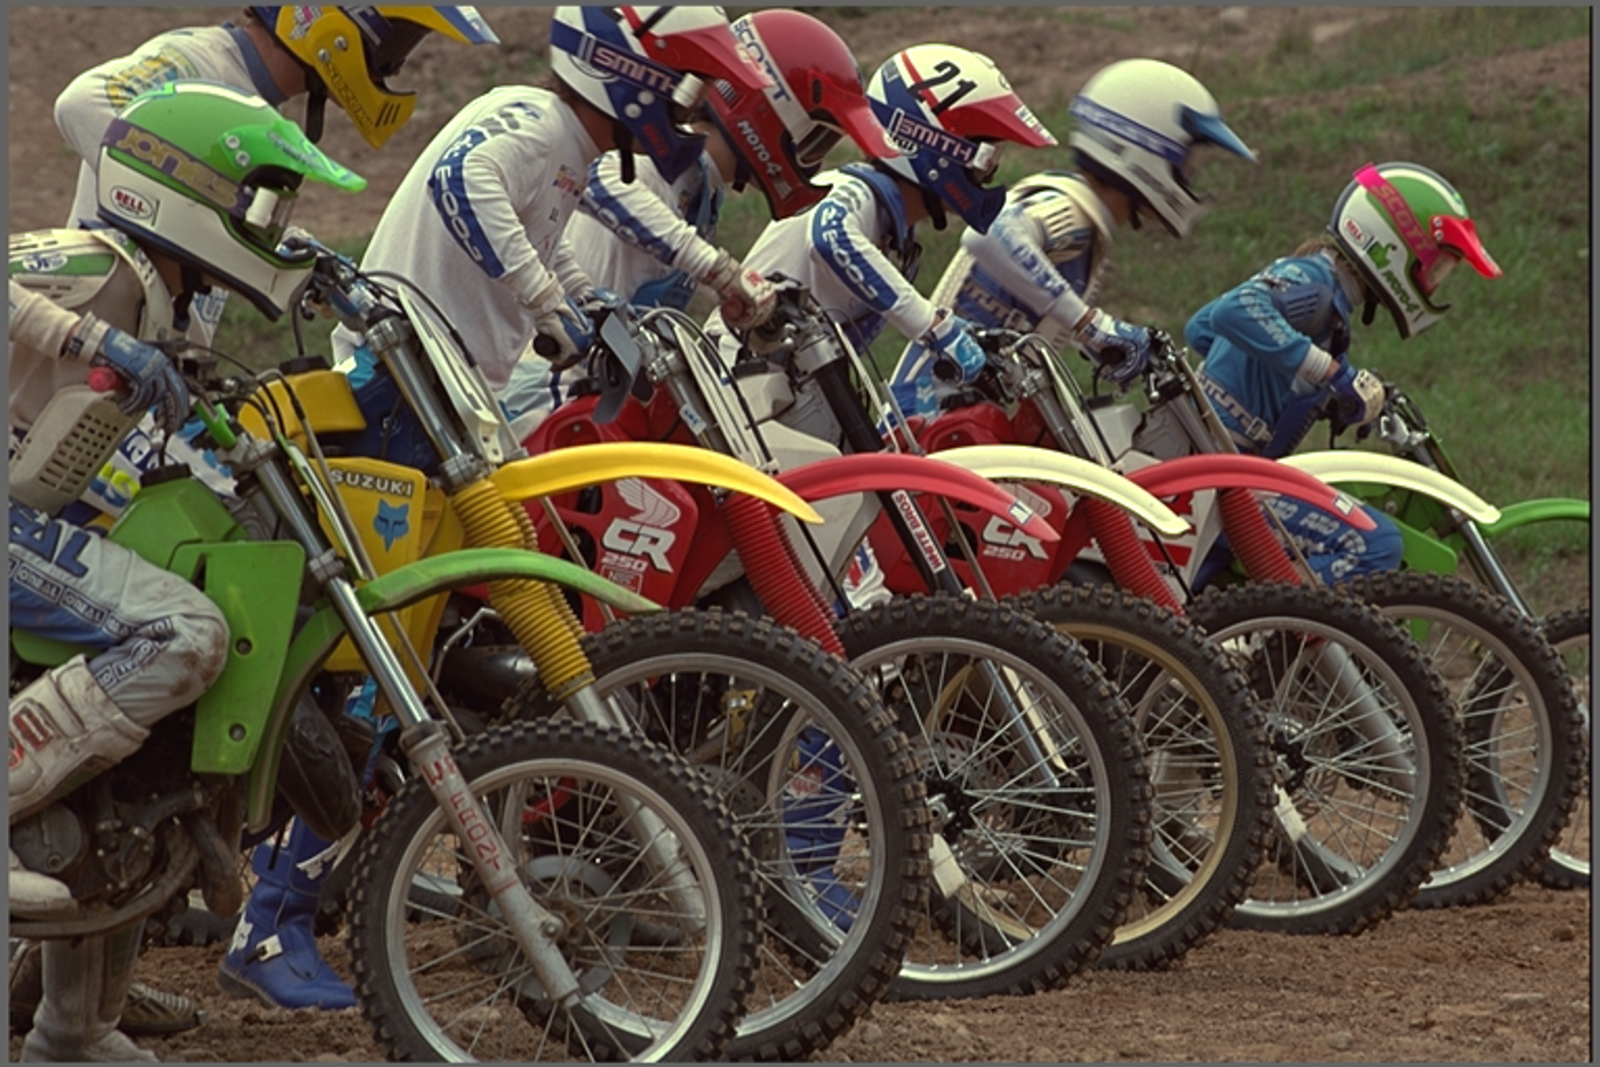
\includegraphics[width=\textwidth]{Figs/Implementation/bikes.pdf}
        \caption{}\label{fig:}
    \end{subfigure}
    \begin{subfigure}[b]{0.4\textwidth}
        \center
        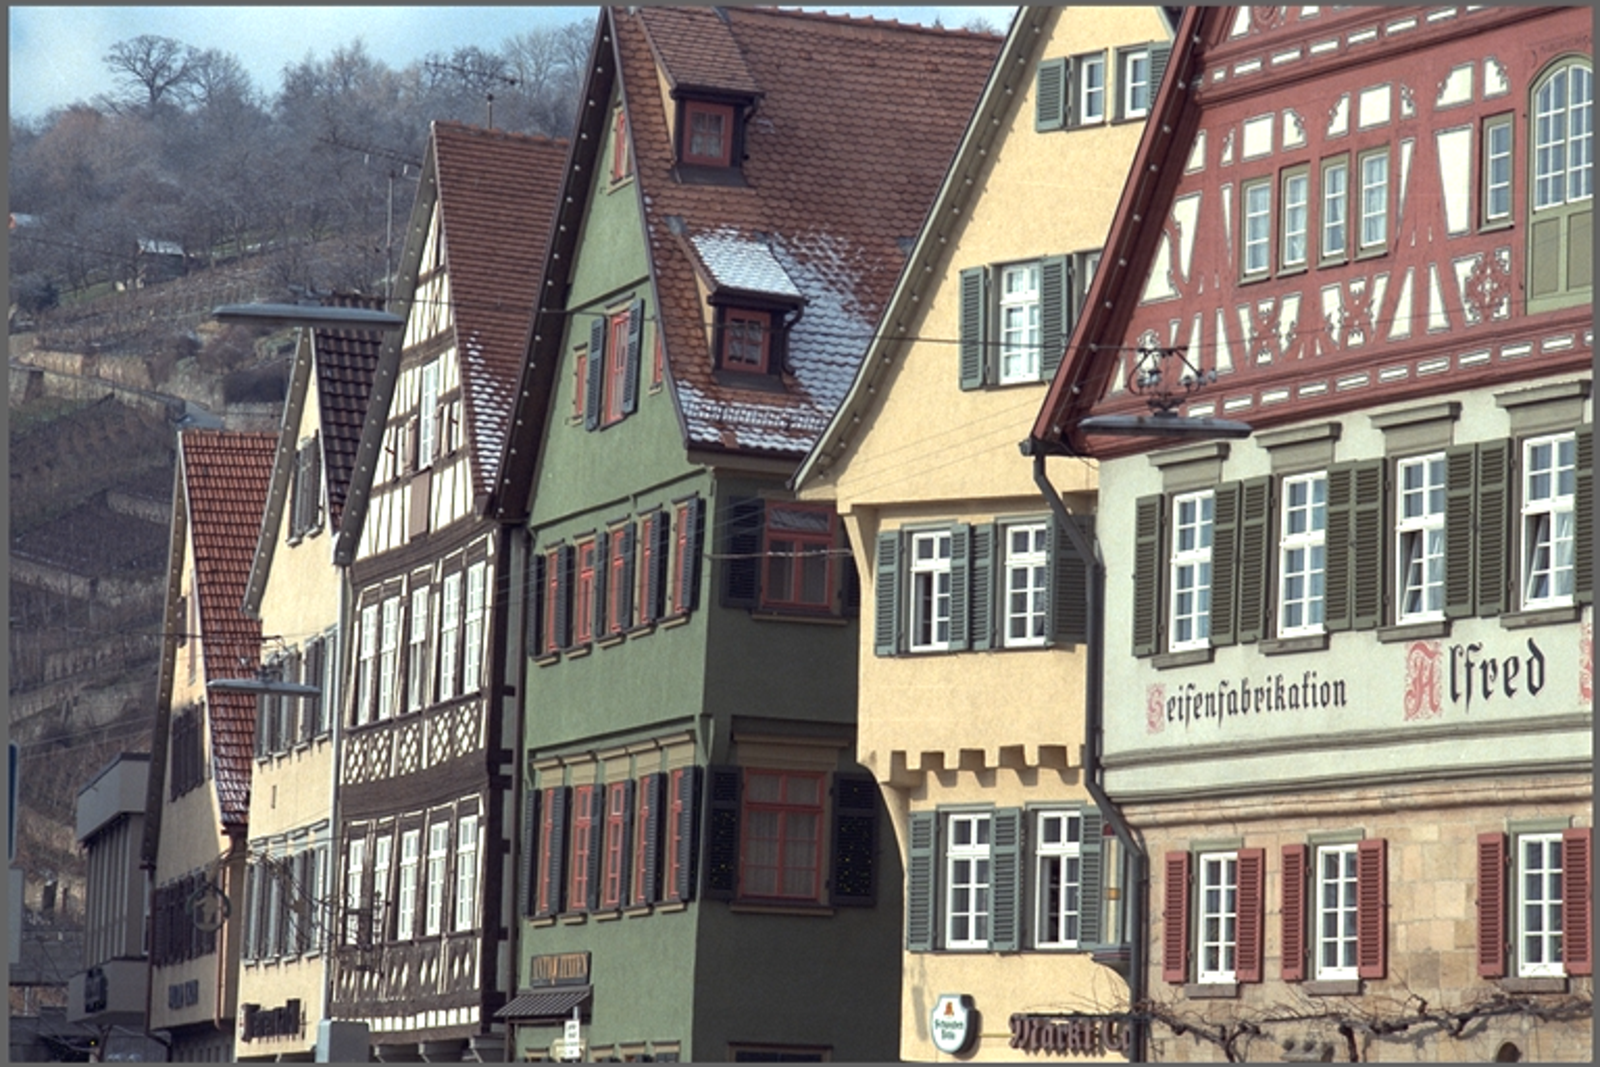
\includegraphics[width=\textwidth]{Figs/Implementation/buildings.pdf}
        \caption{}\label{fig:}
    \end{subfigure}
    \begin{subfigure}[b]{0.4\textwidth}
        \center
        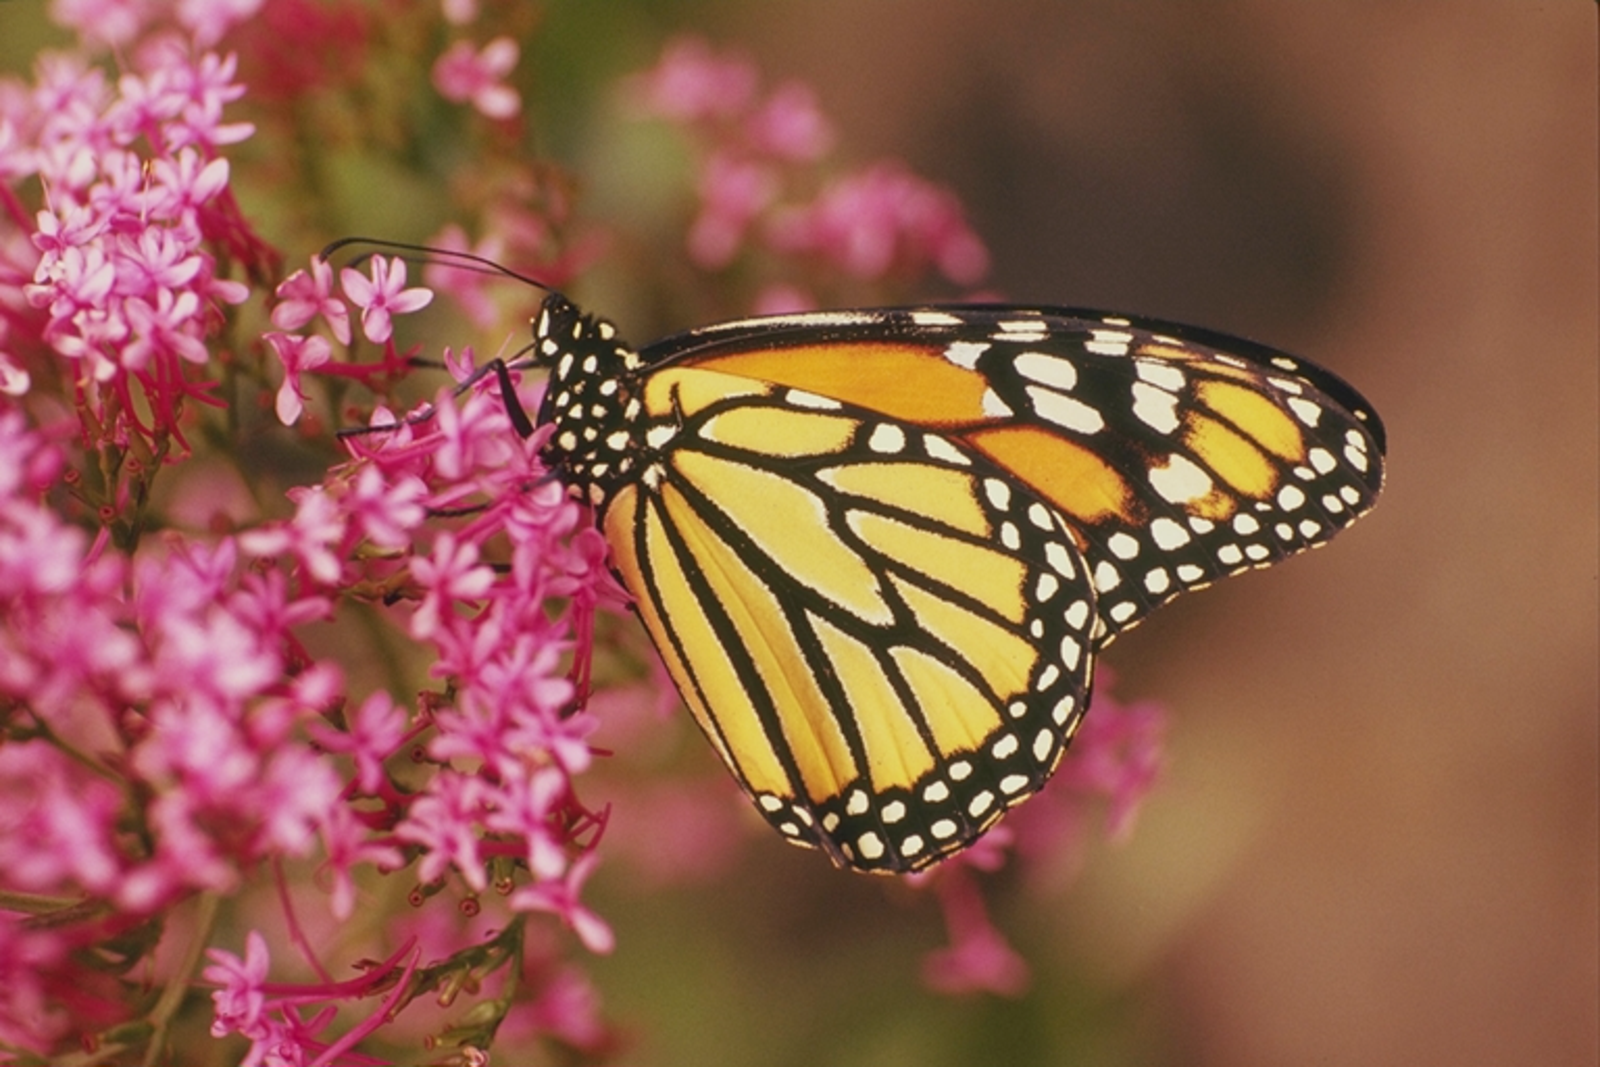
\includegraphics[width=\textwidth]{Figs/Implementation/monarch.pdf}
        \caption{}\label{fig:}
    \end{subfigure}
    \begin{subfigure}[b]{0.4\textwidth}
	    \center
	    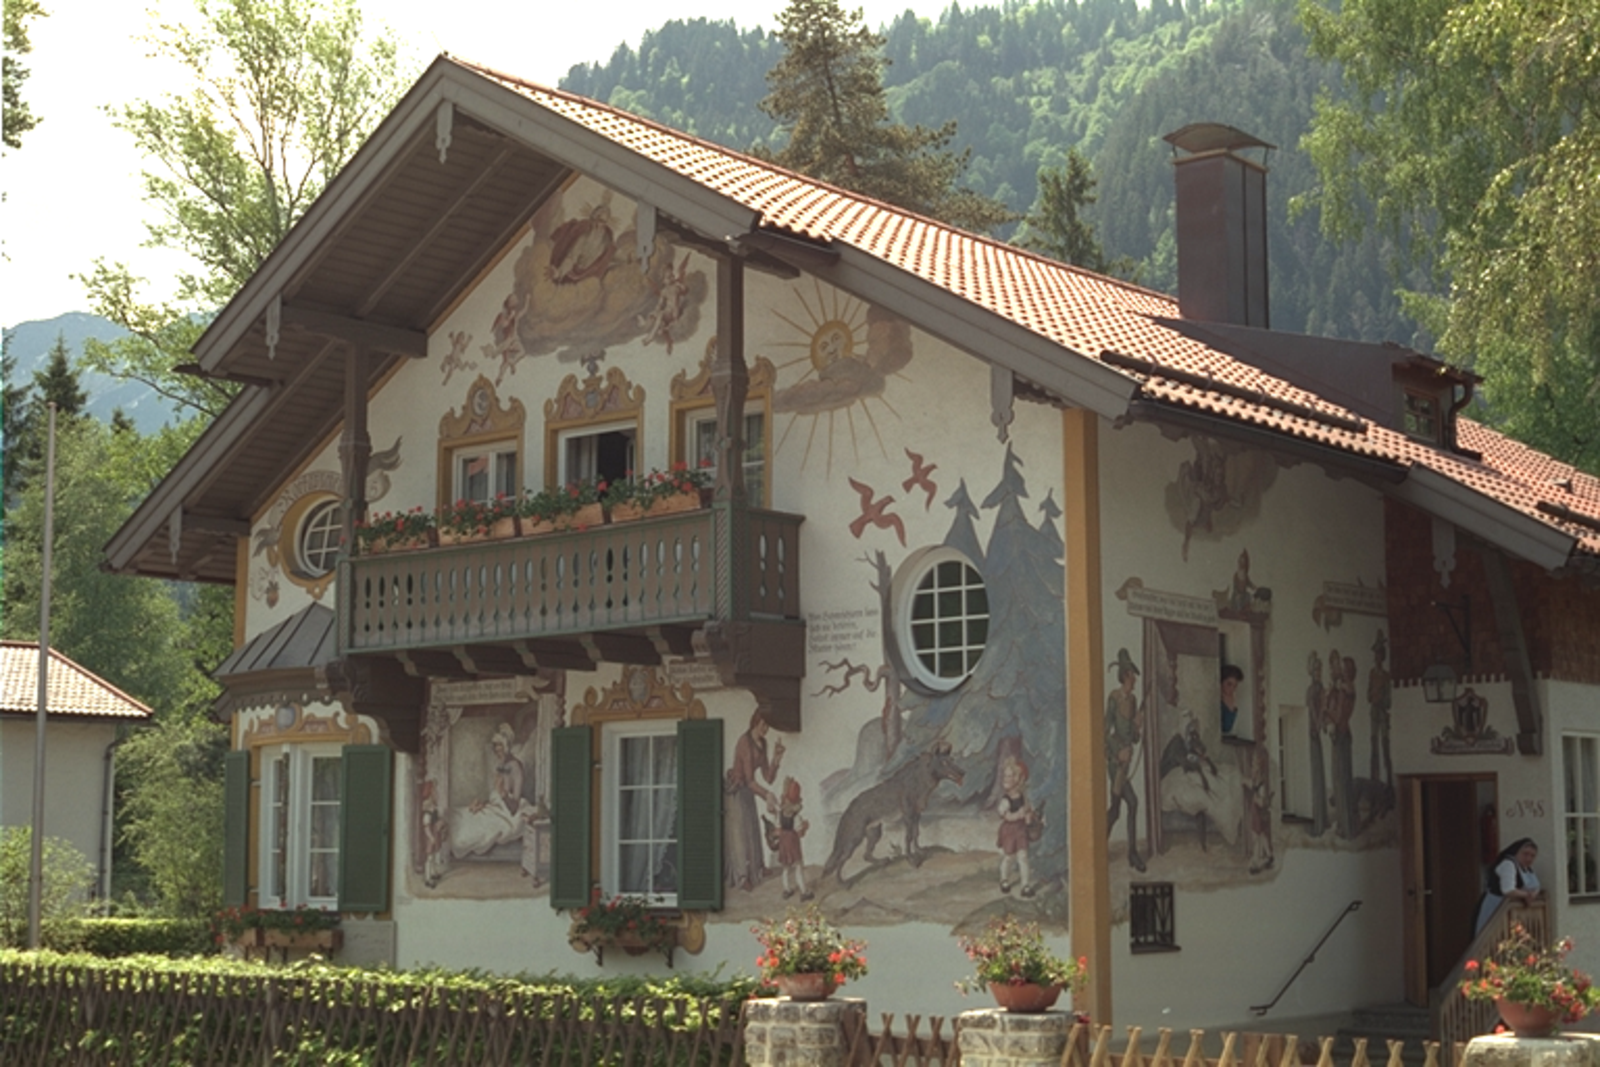
\includegraphics[width=\textwidth]{Figs/Implementation/paintedhouse.pdf}
	    \caption{}\label{fig:}
    \end{subfigure}
    \caption{Examples of reference images from the \gls{live} dataset.}
    \label{fig:live_ex}
\end{figure} 

The five distortions generated from the reference images are Gaussian blur, white noise, JPEG compression, JPEG2K compression and fast fading. By varying the parameters used in creation of the distortions a larger database is created for each type. The total number of images is 982 where 174 are for Gaussian blur, white noise and fast fading. JPEG and JP2K compression have 233 and 227 images respectively. The distorted images were created as follows:

\begin{itemize}
	\item Gaussian blur: blur is added to the images using a circular-symmetric Gaussian kernel of standard deviation $\sigma_B$. The values of $\sigma_b$ are sampled between the range of 0.42 to 15 pixels.
	\item White noise: Gaussian white noise of standard deviation $\sigma_N$ is added to all RGB pixels. Firstly, pixel values are scaled to between 0 and 1. $\sigma_N$ varying between 0.012 and 2.0 is added, afterwards pixel values are rescaled back between 0 and 255.
	\item JPEG compression: compression artefacts are added to the reference bitmap images with JPEG at bit rates between 0.15 \gls{bpp} to 3.34 \gls{bpp}.
	\item JP2K compression: artefacts added ranging between 0.028 \gls{bpp} to 3.15 \gls{bpp}.
	\item Fast fading: this distortions represents errors that can occur when a JP2K bitstream is transmitted over a wireless channel. The receiver signal-to-noise-ratio is varied between 15.5 to 26.1dB for bit errors.
\end{itemize}

Subjective image quality values were calculated by showing human subjects all images, including reference images, and asking them to rate the image as either bad, poor, fair, good, or excellent. The rating was done using a slider on a graphical interface with the five possibilities being evenly spaced. A value between [1, 100] was then found depending on where the subject paced their rating. \gls{dmos} were calculated for each image and averaged between all users for the final image quality annotation for an image. A low \gls{dmos} represents high image quality and a high \gls{dmos} is a low quality image. \figref{gb_ex} shows an example of an image with four varying levels of Gaussian blur and their \gls{dmos} values.

\begin{figure}[H]
    \centering
    \begin{subfigure}[b]{0.4\textwidth}
        \center
        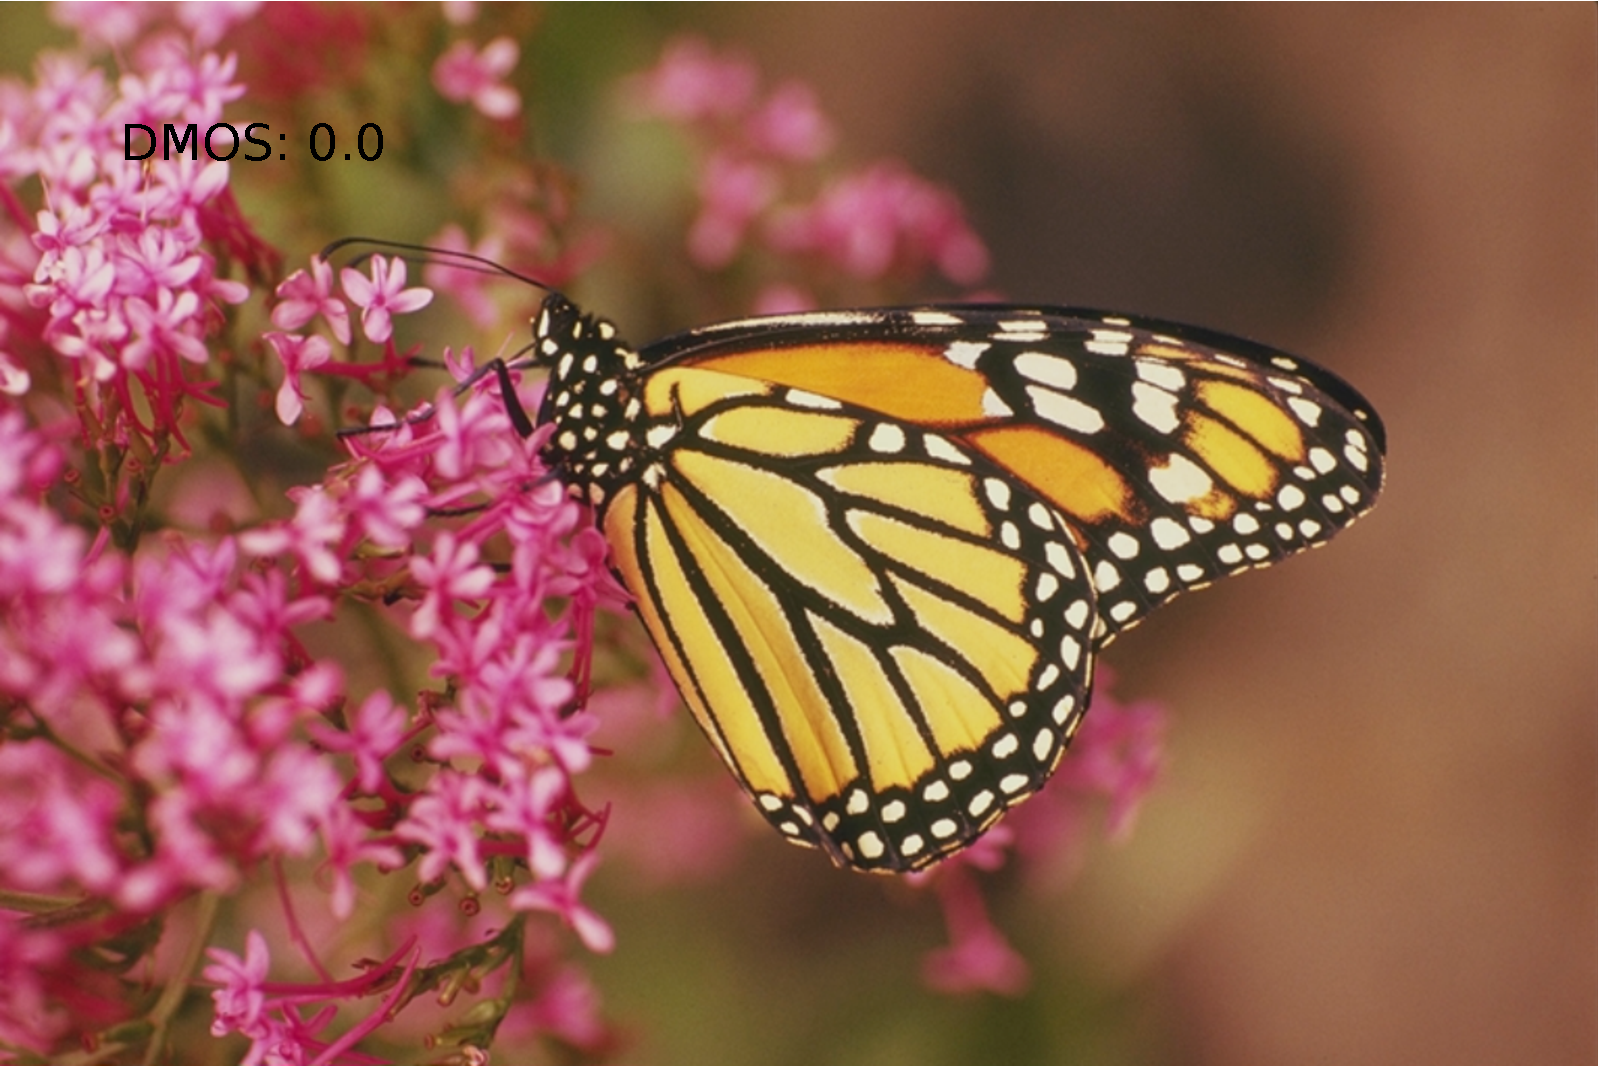
\includegraphics[width=\textwidth]{Figs/Implementation/img173.pdf}
        \caption{\gls{dmos}: 0.0}\label{fig:}
    \end{subfigure}
    \begin{subfigure}[b]{0.4\textwidth}
        \center
        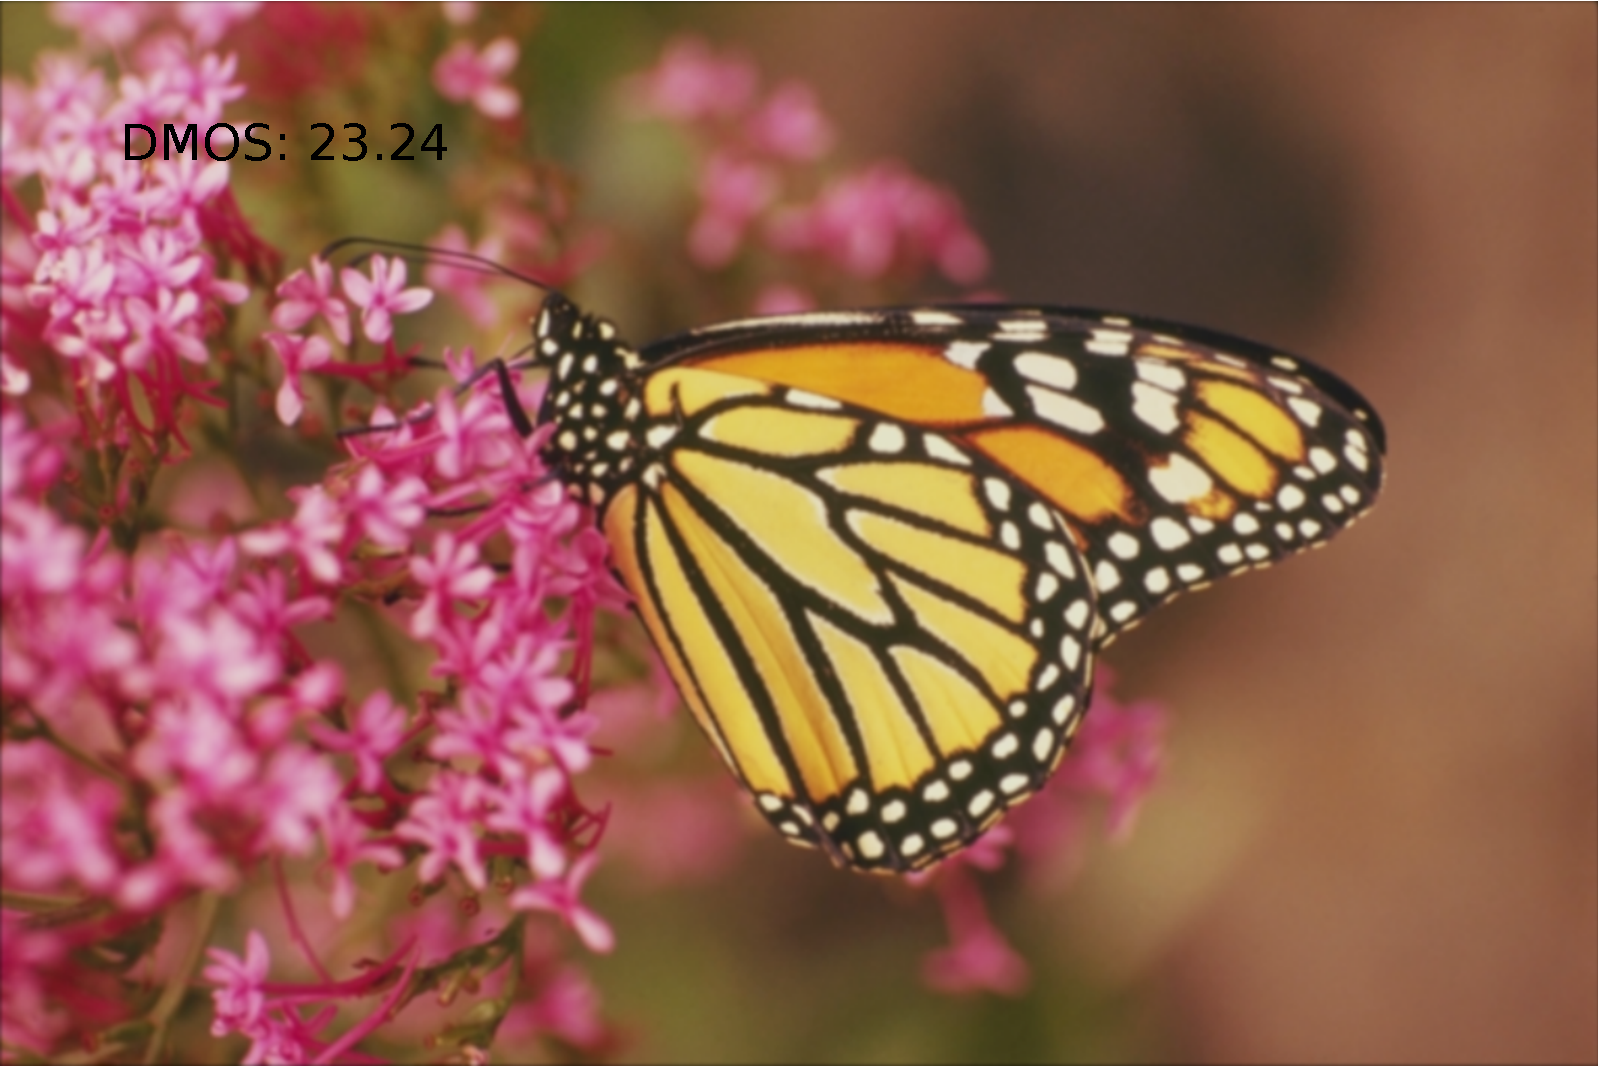
\includegraphics[width=\textwidth]{Figs/Implementation/img96.pdf}
        \caption{\gls{dmos}: 23.24}\label{fig:}
    \end{subfigure}
    \begin{subfigure}[b]{0.4\textwidth}
        \center
        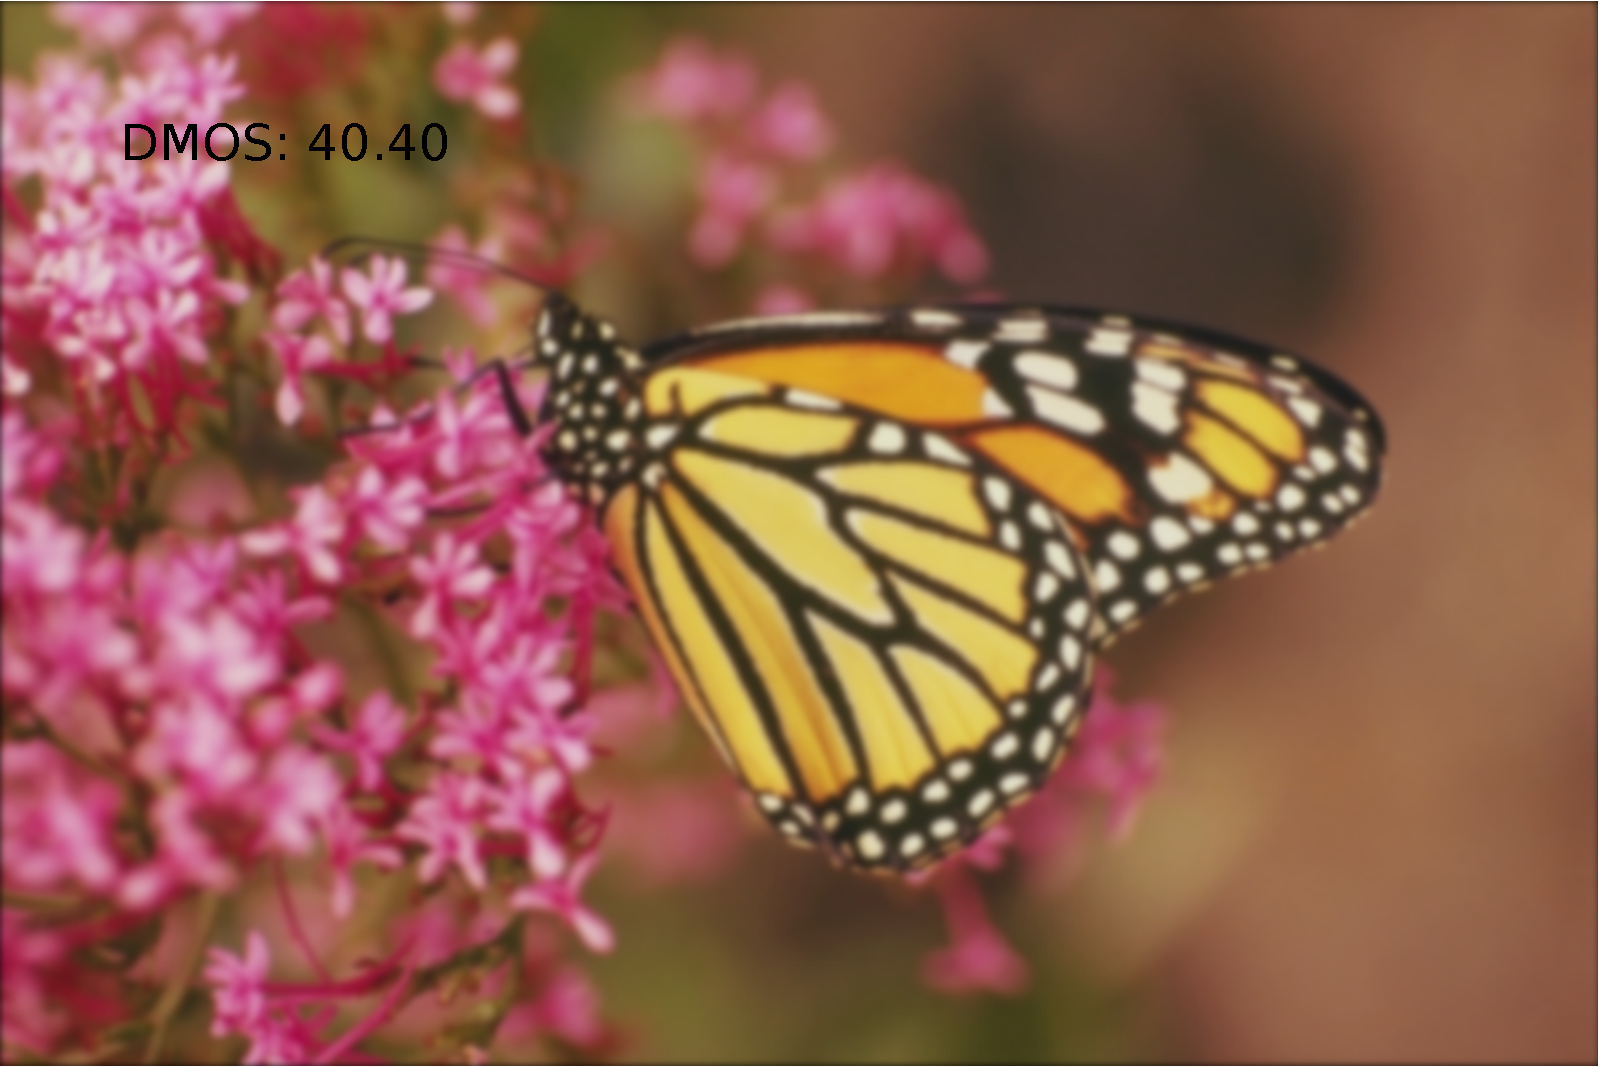
\includegraphics[width=\textwidth]{Figs/Implementation/img103.pdf}
        \caption{\gls{dmos}: 40.40}\label{fig:}
    \end{subfigure}
    \begin{subfigure}[b]{0.4\textwidth}
	    \center
	    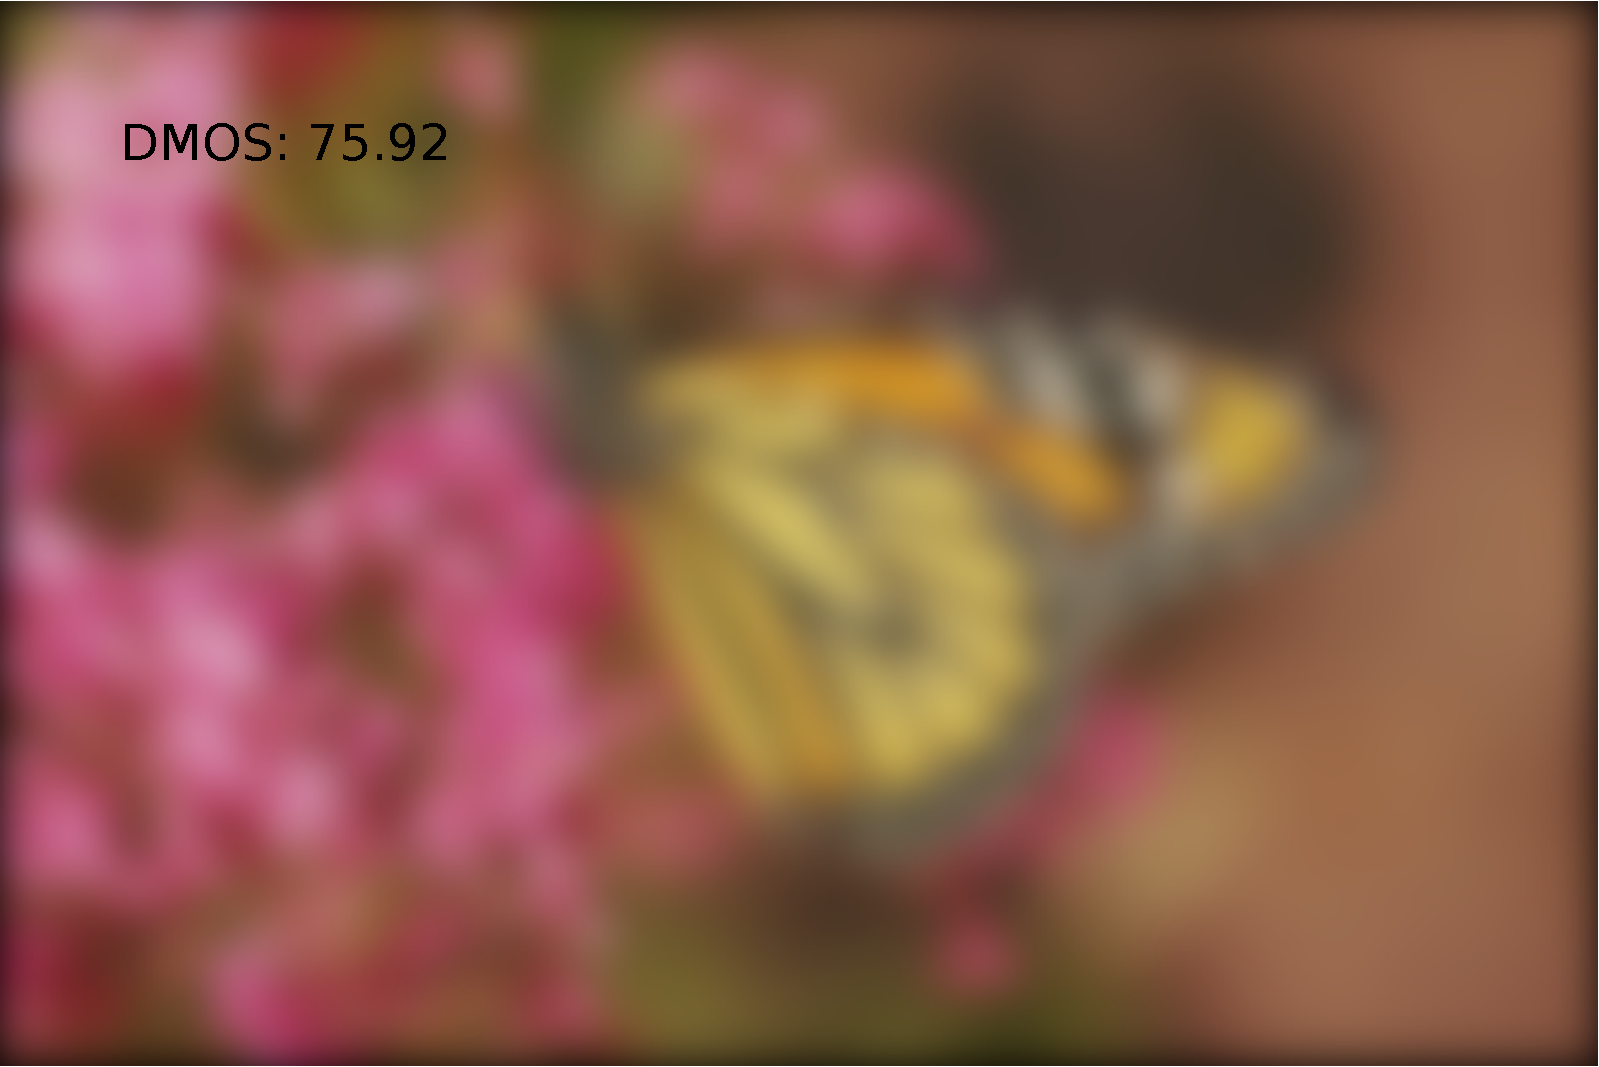
\includegraphics[width=\textwidth]{Figs/Implementation/img11.pdf}
	    \caption{\gls{dmos}: 75.92}\label{fig:}
    \end{subfigure}
    \caption{Four example images from the distortion set. Respective \gls{dmos} scores are shown on the image and below.}
    \label{fig:gb_ex}
\end{figure} 

Given the annotated \gls{dmos} values a system can be trained to predict the image quality of an image. The following section will outline how to train Deep IQA for this purpose.

\subsection{Training Deep IQA}
As per the original authors \cite{deepiqa}, the models are trained for each distortion type in the \gls{live} \gls{iqa} second release dataset \cite{livepaper} \cite{liveweb}. In the original work the Deep IQA model is trained for all five distortion types present in \gls{live}. While this can provide insights into general image quality, individual models are needed to create a more powerful ensemble. The \gls{nr} model was provided by the authors and by taking advantage of the fine-tuning technique, models for each of the individual distortions can be trained in a timely manner. Fine-tuning takes a previously trained model and uses these parameters as a starting point, rather than other commonly used initialisation techniques such as using a Gaussian distribution. As the model is already trained towards all distortions the assumption can be made that only a shorter training cycle is necessary to the new task. The five fine-tuned models are trained in a similar manner to that of the provided model following the guidelines in the original work \cite{deepiqa}. 
\\\\
In the \gls{live} dataset there are 29 reference images from where the respective distortions have been created. When training, the reference images are split into 17 training images, 6 validation images and 6 test images. The deep IQA models are trained using mini-batches consisting of a total of 128 patches per forward/backward pass. The patches are sampled from four randomly selected images from the training split and each image accounts for 32 of the 128 patches in the mini-batch. This process is continued until no more patches are available for mini-batch sampling. This constitutes a completed epoch and all patches are again available for the next epoch. The model provided by the authors was trained for 3,000 epochs, however, as mentioned fine-tuning can drastically reduce the number of epochs required. Therefore, the models for the five distortions are trained for only 500 epochs. The optimisation method for parameter updates is Adam \cite{adam} \add[inline]{explanation of adam solver}. The optimisation settings for Adam are unchanged to that of those used in training the original model. They are as $\beta_1$ = 0.9, $\beta_2$ = 0.999, $\epsilon$ = 10$^{-8}$ and $\alpha$ = 10$^{-4}$. A total of 10 models are trained for each distortion type, each on their individual random split of the 29 reference images. After each of the 500 epochs the model is evaluated on the validation set and the epoch with the best performance is chosen as the final model for testing. The evaluation metrics used for both the validation and test set is \gls{lcc} and \gls{srocc}.\gls{lcc} is used for prediction accuracy as it is a measure of the linear correlation between two sets of data. \gls{srocc} evaluates the prediction monotonicity by measuring the rank correlation between the two sets. For both metrics a value of +1 indicates a positive correlation, 0 is no correlation, and -1 is a negative correlation.
\\\\
The mean results for each of the distortion types can be seen in \tableref{iqaavg}. Each best performing model on the respective validation sets are run on the testing sets and averaged. \add[inline]{add results for all model}

\begin{table}[h]
\centering
\caption{Average Results}
\label{tab:iqaavg}
\begin{tabular}{|l|l|l|}
\hline
Distortion Type & LCC    & SROCC  \\ \hline
Gaussian Blur   & 0.9750 & 0.9681 \\ \hline
White Noise     & 0.9957 & 0.9887 \\ \hline
JPEG            & 0.9805 & 0.9523 \\ \hline
JP2K            & 0.9788 & 0.9600 \\ \hline
FF     & 0.9679 & 0.9505 \\ \hline
\end{tabular}
\end{table}


\subsection{PASCAL VOC Data Split}
Each model for the five distortion types and run through the 07++12 dataset in order to give an indication to the respective distributions, as done for the object sizes in \sectionref{resawareSec}. The distributions can been seen in the histograms in \figref{iqdist}.

\begin{figure}[H]
    \centering
    \begin{subfigure}[b]{0.4\textwidth}
        \center
        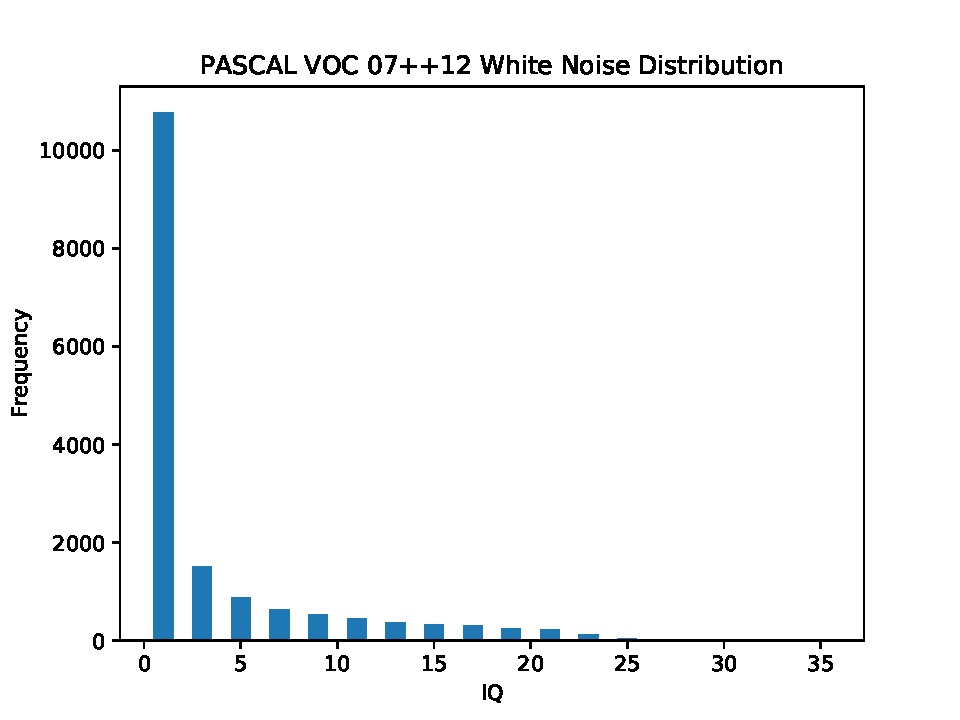
\includegraphics[width=\textwidth]{Figs/Implementation/WhiteNoisedist.pdf}
        \caption{}\label{fig:dist_wn}
    \end{subfigure}
    \begin{subfigure}[b]{0.4\textwidth}
        \center
        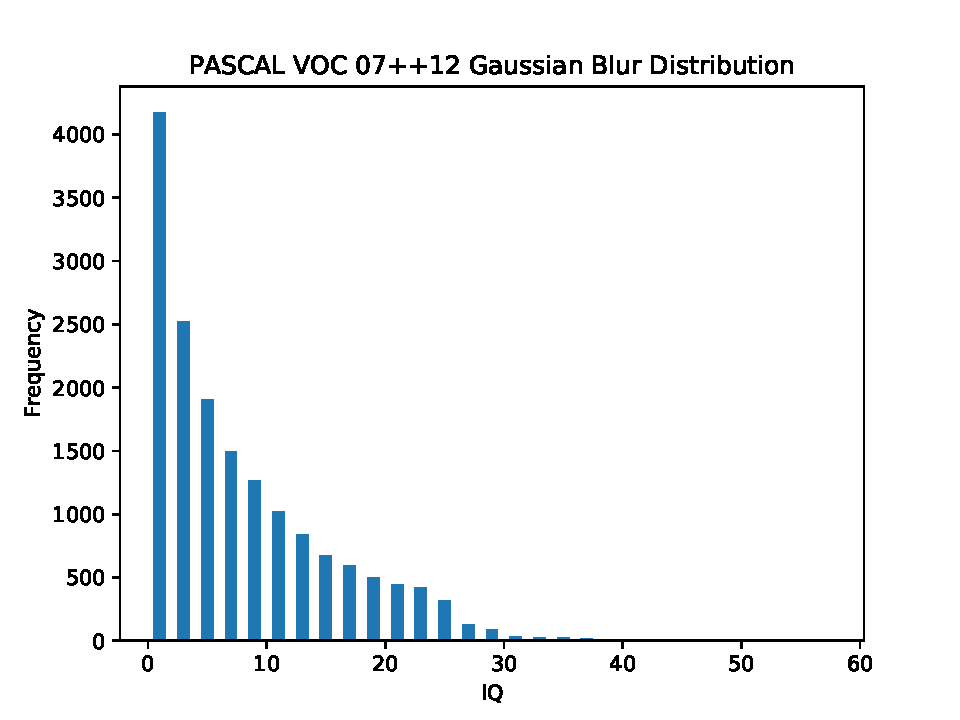
\includegraphics[width=\textwidth]{Figs/Implementation/GaussianBlurdist.pdf}
        \caption{}\label{fig:dist_gb}
    \end{subfigure}
    \begin{subfigure}[b]{0.4\textwidth}
        \center
        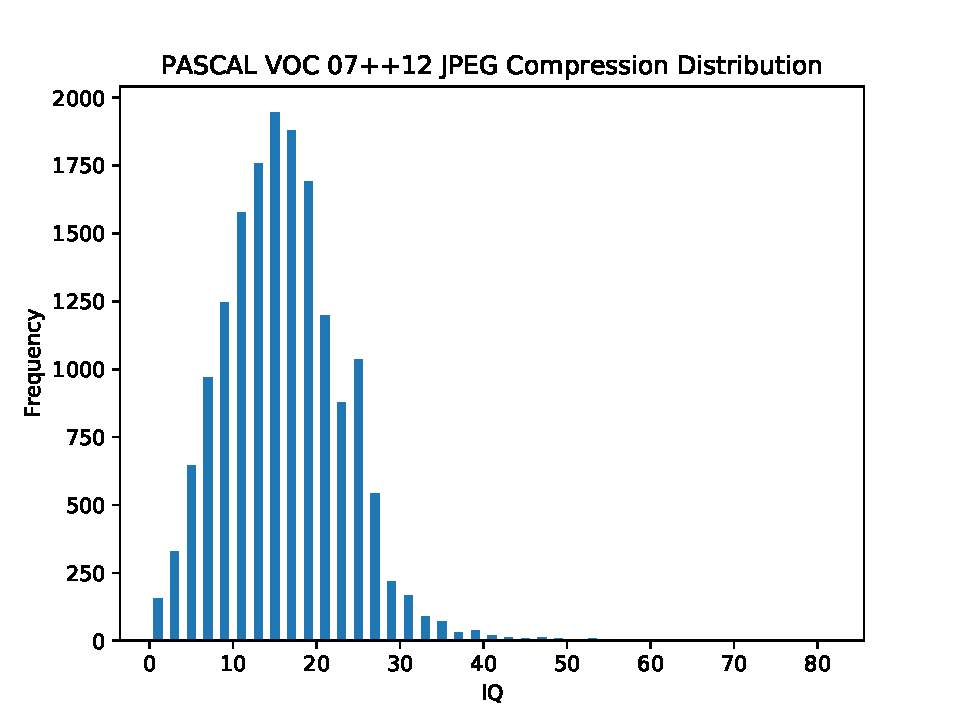
\includegraphics[width=\textwidth]{Figs/Implementation/JPEGCompressiondist.pdf}
        \caption{}\label{fig:dist_jp}
    \end{subfigure}
    \begin{subfigure}[b]{0.4\textwidth}
        \center
        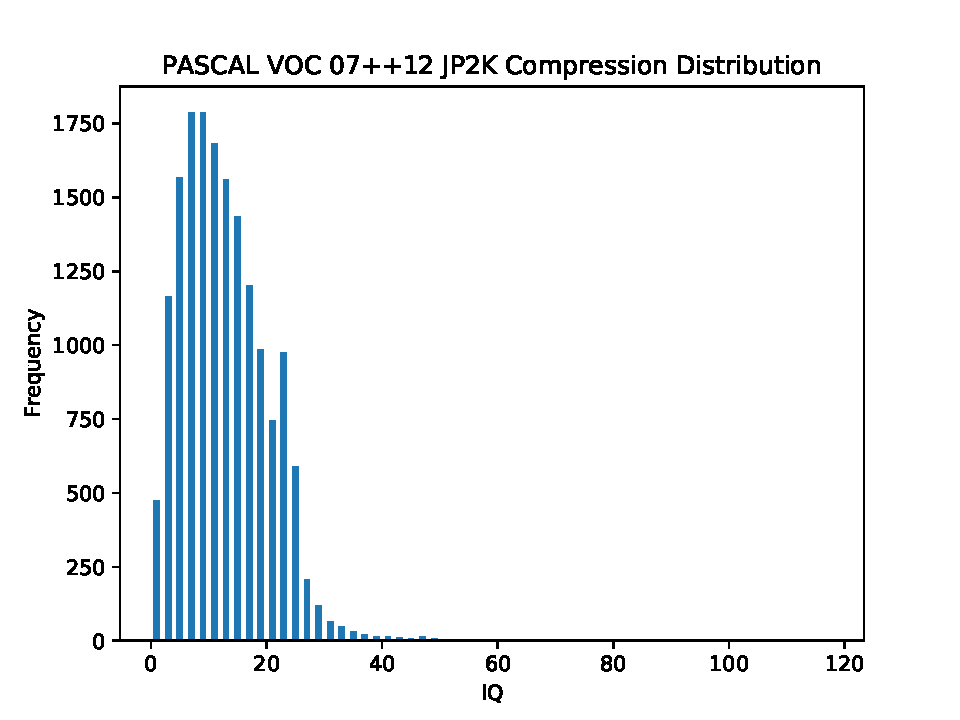
\includegraphics[width=\textwidth]{Figs/Implementation/JP2KCompressiondist.pdf}
        \caption{}\label{fig:dist_jk}
    \end{subfigure}
  	\begin{subfigure}[b]{0.4\textwidth}
        \center
        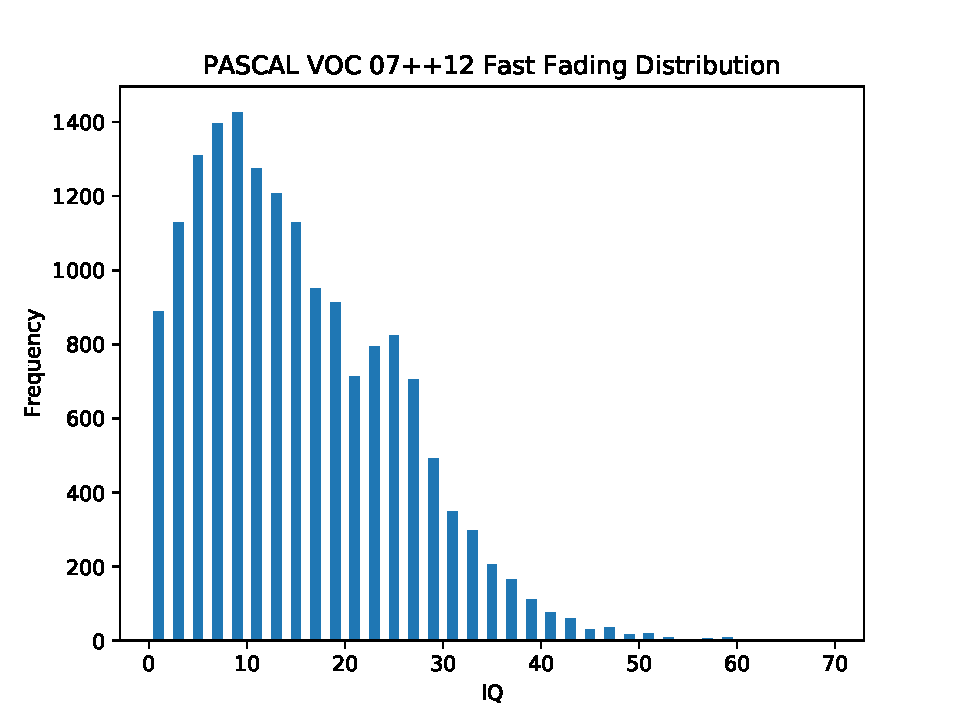
\includegraphics[width=\textwidth]{Figs/Implementation/FastFadingdist.pdf}
        \caption{}\label{fig:dist_ff}
    \end{subfigure}
    \caption{Histograms representing the distribution of image quality for the five distortions trained from the \gls{live} image quality dataset. The distortions shown are white noise (a), Gaussian blur (b), JPEG compression (c), JP2k compression (d), fast fading (e).}
    \label{fig:iqdist}
\end{figure} 

The distribution for white noise and Gaussian blur is skewed towards a higher image quality as seen in \figref{dist_wn} and \figref{dist_gb} and also to a lesser extent in fast fading in \figref{dist_ff}. Whereas the image quality for compression distortions is somewhat of a Gaussian nature in \figref{dist_jp} and \figref{dist_jk}. For determining an appropriate manner to split the data the same constraints are made as in that for object sizes, namely that both subsets of data should have an equal number of ground truths to train on. Again by taking the median for each of the five distributions can satisfy this. The respective medians can be seen in \tableref{iq_splits}.

\begin{table}[h]
\centering
\caption{My caption}
\label{tab:iq_splits}
\begin{tabular}{|l|l|}
\hline
\textbf{Distortion Type}   & \textbf{Median} \\ \hline
White Noise       & 0.599  \\ \hline
Gaussian Blur     & 5.607  \\ \hline
JPEG Compression  & 15.660 \\ \hline
JP2K Compression & 11.747 \\ \hline
Fast Fading       & 13.373 \\ \hline
\end{tabular}
\end{table}

A skewed distribution of data was also present for object sizes, however, creating two subsets of data for high and low white noise image quality does not appear to be feasible. The combination of both the heavy skew and half of the data lying below 0.599 indicates that a minimal amount of white noise distortion is present in the 07++12 dataset. Therefore, this distortion is not considered for part of the ensemble. While the Gaussian blur image quality is also skewed it is similar to that of the the object sizes and therefore is deemed appropriate to split based upon its median of 5.607. The remaining distributions are much less skewed and therefore a total of eight R-FCN models will be trained for the high and low levels of image quality for the distortions Gaussian blur, JPEG compression, JP2K compression and fast fading. Therefore, in total there will be ten R-FCN models trained including the two for smaller and larger object sizes.
\\\\
The 07++12 dataset has a total of 16,551 images and as this data is to be distributed into eight different subsets there is a possibility that there is a high level of overlap between the sets. As the aim of the ensemble is to learn to detect objects based upon different information, if subsets are two similar there may be potentially no advantage gained between two or more models. Therefore, a comparison matrix is used to evaluate how much the different combinations of 07++12 match. This can be seen for higher quality subsets in \tableref{highcomp}, lower quality in \tableref{lowcomp} and between lower and higher quality in \tableref{lowhighcomp}.

\begin{table}[h]
\centering
\caption{Higher Quality}
\label{tab:highcomp}
\begin{tabular}{|l|l|l|l|l|}
\hline
             & \textbf{Gaussian Blur}  & \textbf{JPEG} & \textbf{JP2K} & \textbf{FF}    \\ \hline
\textbf{Gaussian Blur} &                & 74.14\% & 70.78\% & 83.12\% \\ \hline
\textbf{JPEG}   & 74.14\% &                & 80.62\% & 77.98\% \\ \hline
\textbf{JP2K}   & 70.78\%  & 80.62\% &                & 72.75\% \\ \hline
\textbf{FF}   & 83.12\% & 77.98\% & 72.75\% &                \\ \hline
\end{tabular}
\end{table}

\begin{table}[h]
\centering
\caption{Lower Quality}
\label{tab:lowcomp}
\begin{tabular}{|l|l|l|l|l|}
\hline
             & \textbf{Gaussian Blur}  & \textbf{JPEG} & \textbf{JP2K} & \textbf{FF}     \\ \hline
\textbf{Gaussian Blur}  &                & 74.14\%   & 70.78\% & 83.11\% \\ \hline
\textbf{JPEG}    & 74.14\% &                & 80.62\% & 77.98\% \\ \hline
\textbf{JP2K}   & 70.78\% & 80.62\% &                & 72.75\% \\ \hline
\textbf{FF}  & 83.11\% & 77.98\% & 72.75\% &                \\ \hline
\end{tabular}
\end{table}

For the subsets of data for both higher and lower quality there are a few instances of relatively high overlap in images. The largest is between \gls{ff} \add[inline]{gls for FF} and Gaussian blur with 83.12\% and 83.11\%. Other instances of overlap also appears between JPEG and JP2K compression which could be intuitively explained due to their similarities in their distortions. However, in general it is deemed that enough difference is present between the splits to train variants of R-FCN networks.

Finally, \tableref{lowhighcomp} shows the comparison matrix between all eight data subsets. There is much less overlap between these sets as much of the overlaps are present in respective higher and lower configurations as seen in \tableref{highcomp} and \tableref{lowcomp}.

\begin{table}[]
\centering
\caption{Lower / Upper}
\label{tab:lowhighcomp}
\begin{tabular}{|l|l|l|l|l|}
\hline
                 & \textbf{Gaussian Blur$_{Lower}$} & \textbf{JPEG$_{Lower}$} & \textbf{JP2K$_{Lower}$} & \textbf{FF$_{Lower}$} \\ \hline
\textbf{Gaussian Blur$_{Higher}$}  & 0\%             & 25.86\% & 29.22\% & 16.88\%    \\ \hline
\textbf{JPEG$_{Higher}$} & 25.86\%      & 0\%        & 19.38\% & 22.02\%    \\ \hline
\textbf{JP2K$_{Higher}$} & 29.22\%      & 19.38\% & 0\%        & 27.25\%    \\ \hline
\textbf{FF$_{Higher}$} & 16.88\%      & 22.02\% & 27.25\% & 0\%           \\ \hline
\end{tabular}
\end{table}

%%%%%%%%5
\begin{comment}

	\begin{table}[h]
	\centering
	\caption{Lower}
	\label{my-label}
	\begin{tabular}{|l|l|l|l|l|l|}
	\hline
	              & White Noise    & Gaussian Blur  & JPEG           & JP2K           & Fast Fading    \\ \hline
	White Noise   &                & 3511 / 42.42\% & 2918 / 35.25\% & 2263 / 27.34\% & 3722 / 44.97\% \\ \hline
	Gaussian Blur & 3511 / 42.42\% &                & 6136 / 74.14\% & 5858 / 70.78\% & 6879 / 83.12\% \\ \hline
	JPEG          & 3511 / 42.42\% & 6136 / 74.14\% &                & 6672 / 80.62\% & 6454 / 77.98\% \\ \hline
	JP2K          & 2263 / 27.34\% & 5857 / 70.78\%  & 6672 / 80.62\% &                & 6021 / 72.75\% \\ \hline
	Fast Fading   & 3722 / 44.97\% & 6879 / 83.12\% & 6454 / 77.98\% & 6021 / 72.75\% &                \\ \hline
	\end{tabular}
	\end{table}

	\begin{table}[h]
	\centering
	\caption{Upper}
	\label{my-label}
	\begin{tabular}{|l|l|l|l|l|l|}
	\hline
	              & White Noise    & Gaussian Blur  & JPEG           & JP2K           & Fast Fading    \\ \hline
	White Noise   &                & 3510 / 42.17\% & 2917 / 35.25\% & 2262 / 27.34\% & 3721 / 44.96\% \\ \hline
	Gaussian Blur & 3510 / 42.17\% &                & 6135 74.14\%   & 5857 / 70.78\% & 6878 / 83.11\% \\ \hline
	JPEG          & 2917 / 35.25\% & 6135 / 74.14\% &                & 6671 / 80.62\% & 6453 / 77.98\% \\ \hline
	JP2K          & 2262 / 27.34\% & 5857 / 70.78\% & 6671 / 80.62\% &                & 6020 / 72.75\% \\ \hline
	Fast Fading   & 3721 / 44.96\% & 6878 / 83.11\% & 6453 / 77.98\% & 6020 / 72.75\% &                \\ \hline
	\end{tabular}
	\end{table}

	\begin{table}[]
	\centering
	\caption{Lower / Upper}
	\label{my-label}
	\begin{tabular}{|l|l|l|l|l|l|}
	\hline
	                    & White Noise Upper & Gaussian Blur Upper & JPEG Upper     & JP2K Upper     & Fast Fading Upper \\ \hline
	White Noise Lower   & 0 / 0\%           & 4765 / 57.57\%      & 5358 / 64.74\% & 6013 / 72.66\% & 4554 / 55.03\%    \\ \hline
	Gaussian Blur Lower & 4756 / 57.58\%    & 0 / 0\%             & 2140 / 25.86\% & 2418 / 29.22\% & 1397 / 16.88\%    \\ \hline
	JPEG Lower          & 5358 / 64.74\%    & 2140 / 25.86\%      & 0 / 0\%        & 1604 / 19.38\% & 1822 / 22.02\%    \\ \hline
	JP2K Lower          & 6013 / 72.66\%    & 2418 / 29.22\%      & 1604 / 19.38\% & 0 / 0\%        & 2255 / 27.25\%    \\ \hline
	Fast Fading Lower   & 4554 / 55.03\%    & 1397 / 16.88\%      & 1822 / 22.02\% & 2255 / 27.25\% & 0 / 0\%           \\ \hline
	\end{tabular}
\end{table}
\end{comment}


\begin{comment}
	Results of training Deep IQA for LIVE distortions
	- given model trained on all distortion types in LIVE dataset provided by the authors, finetune to each of the 5 distortions
		- trained for 500 epochs in same training style as Deep IQA
	- best model for each distortion type for further work determined by average of LCC and SROCC for each model
	- these are as follows:
		- GB: 5 - 0.98885
		- WN: 7 - 0.9964
		- JPEG: 7 - 0.974
		- JP2K: 6 - 0.98445
		- FF: 6 - 0.9798

\end{comment}